% Chapter 1

\chapter{Introducción general} % Main chapter title

\label{Chapter1} % For referencing the chapter elsewhere, use \ref{Chapter1} 
\label{IntroGeneral}
En este capítulo se presentan las características de los robots de servicio, se  reseña el uso de luz ultravioleta como germicida y se exponen los objetivos que motivaron el presente trabajo y sus respectivo alcance.
%----------------------------------------------------------------------------------------

% Define some commands to keep the formatting separated from the content 
\newcommand{\keyword}[1]{\textbf{#1}}
\newcommand{\tabhead}[1]{\textbf{#1}}
\newcommand{\code}[1]{\texttt{#1}}
\newcommand{\file}[1]{\texttt{\bfseries#1}}
\newcommand{\option}[1]{\texttt{\itshape#1}}
\newcommand{\grados}{$^{\circ}$}

%----------------------------------------------------------------------------------------

%\section{Introducción}

%----------------------------------------------------------------------------------------
\section{Robots de servicio}

A lo largo del siglo XX la robótica pasó de ser una temática de la rama de la ciencia ficción, a cumplir un importante rol dentro de los complejos industriales. En los últimos años los robots han pasado a tener cada vez más tareas de “servicio” para ambientes  públicos y hogareños.
La robótica de servicios abarca un amplio campo de aplicaciones, la mayoría de las cuales tienen diferentes grados de automatización, desde la teleoperación completa hasta la funcionamiento autónomo, y constituye un campo de aplicación más diverso que el de la robótica industrial. En la  figura \ref{fig:robotsservicio} se pueden observar tres tipos de robots de servicios: una aspiradora hogareña, un cortador de césped y un limpiavidrios.

\begin{figure}[h]
	\centering
	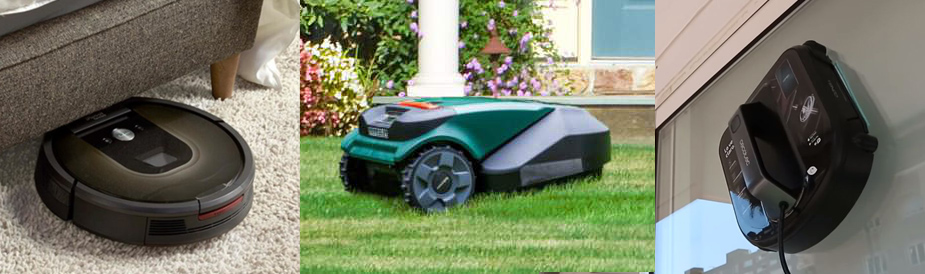
\includegraphics[width=\textwidth]{./Figures/robotsservicio.jpg}
	\caption{robots de servicio.\protect\footnotemark.}
	\label{fig:robotsservicio}
\end{figure}
\footnotetext{Imágenes tomadas de \url{https://www.domotizar.com/}}


A mediados de la década de 1990, la Comisión Económica de las Naciones Unidas para Europa (UNECE) .\citep{UNECE} y la Federación Internacional de Robótica (IFR) .\citep{IFR} adoptaron un sistema de clasificación de robots de servicio dividida por categorías y tipos de interacción, que se ha mantenido clasificación actual. En la  figura \ref{fig:robotsservicio} se puede observar los primeros ítems de clasificación para robots domésticos/personales de acuerdo a los tipos y áreas de aplicación.



\begin{figure}[h]
	\centering
	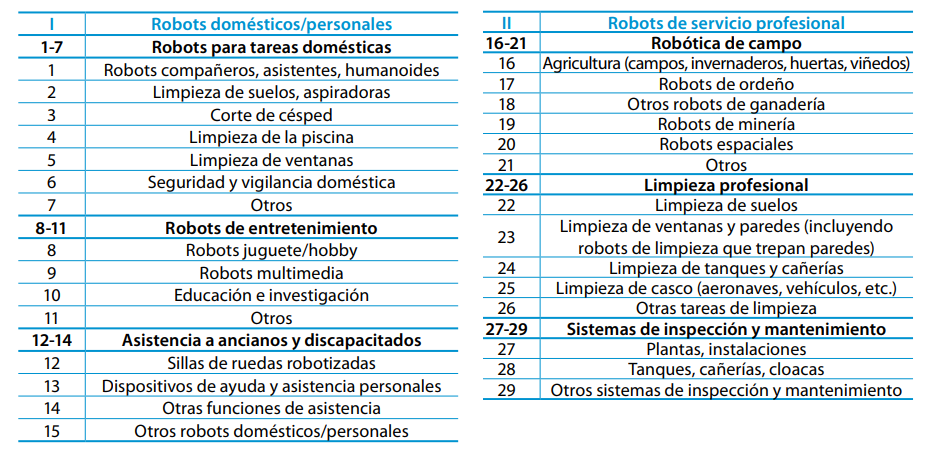
\includegraphics[width=\textwidth]{./Figures/clasificacion.png}
	\caption{clasificación de robots de servicio.\protect\footnotemark.}
	\label{fig:clasificacion}
\end{figure}
\footnotetext{Imagen tomada de \url{https://www.editores-srl.com.ar/sites/default/files/aa1_ifr_robots.pdf}}




\subsection{Robots móviles para inspección y limpieza}

Los robots móviles son dispositivos que poseen un sistema de locomoción capaz de navegar a través de un determinado ambiente de trabajo. Normalmente cuentan con cierto nivel de autonomía que les permite el desplazamiento sin colisiones por un recorrido específico. Sus aplicaciones son muchas y en general  están relacionadas con tareas monótonas o riesgosas para la salud humana.
Las plataformas móviles pueden realizar tareas de inspección y limpieza de manera autónoma o controlada remotamente por un operador. Son utilizadas en zonas de difícil acceso debido a limitaciones de espacio o razones de seguridad.  
Este tipo de robot suele contar con sensores de distinto tipo, para detectar los límites y obstáculos ante los que se presentan. 
La proliferación de de robots para limpieza se incrementó fuertemente a partir de la pandemia de Covid-19, con lo que se los puede encontrar hoy en día en espacios en los que antes no estaban presentes, tales como salas médicas,  hoteles y en el transporte público  .\citep{Cleaning}. Estos dispositivos “de interior” abarcan a la aspiradoras robóticas y a los robots de lavado de pisos que limpian pisos con funciones de barrido y trapeado húmedo. 

%----------------------------------------------------------------------------------------

\subsubsection{Robots de limpieza UVC}

Acá va una comparativa de robots de limpieza UVC.
.
.
.
.
.
%----------------------------------------------------------------------------------------

\subsubsection{Desinfección usando Luz ultravioleta}

El espectro ultravioleta (UV) abarca la banda de radiación electromagnética entre los 400 y 100 nm, presentando una longitud de onda menor que la de la luz visible y mayor que la de los rayos X.  Se divide en tres las siguientes categorías principales: los rayos UV-A (400 – 315 nm), que son los más cercanos al espectro visible; los rayos UV-B (315 – 280 nm), que son absorbidos en gran parte por diferentes elementos a medida que atraviesan el cielo y los rayos UV-C (280 – 200 nm), que son absorbidos totalmente por la capa de ozono. En la  figura \ref{fig:espectro} se observa detalle de parte del espectro de radiación electromagnética y  su clasificación según longitud de onda.


\begin{figure}[h]
	\centering
	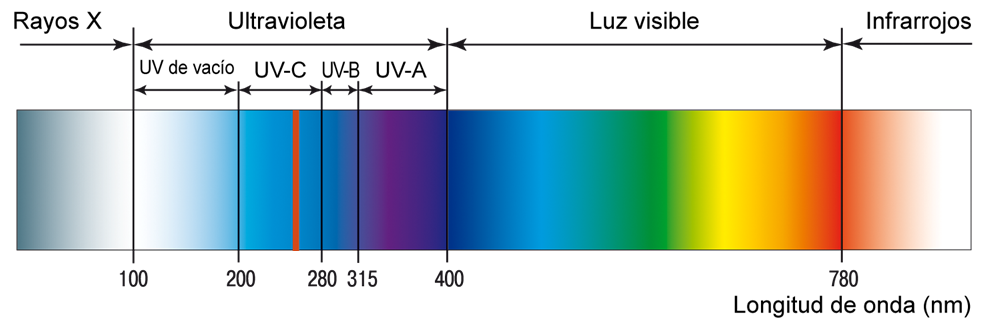
\includegraphics[width=\textwidth]{./Figures/espectro.PNG}
	\caption{clasificación según longitud de onda.\protect\footnotemark.}
	\label{fig:espectro}
\end{figure}
\footnotetext{Imagen tomada de \url{https://www.lit-uv.com/es/technology/}}

La utilización de luz ultravioleta UV-C como germicida ha demostrado efectividad para la esterilización  las bacterias, gérmenes, virus, algas y esporas. 

Los virus tienen un tamaño inferior a un micrómetro (µm, una millonésima parte de un metro) y las bacterias son típicamente de 0,5 a 5 µm. Técnicamente es incorrecto decir que los rayos  UV-C matan a los virus, siendo que no se trata de organismos vivientes. Sin embargo, el comité de foto-biología de la \emph{ Illuminating Engineering Society}(IES) informa que los fotones UV-C interactúan con el ARN y las moléculas de ADN en un virus o bacteria de modo que se evita su reproducción y por lo tanto su efecto infeccioso. A este proceso se lo denomina “desactivación”  \citep{IES}.

La \emph{International Ultraviolet Association}  (IUVA) afirma que los resultados de pruebas en laboratorio de desinfección utilizando UV-C entre los 200 y 280nm demuestran especial utilidad para reducir la transmisión de los virus causantes del COVID-19:  SARS-CoV-1 y MERS-CoV \citep{IUA}. En la práctica, el efecto depende de factores tales como  el tiempo de exposición y obstrucción que puedan tener los rayos para alcanzar plenamente los pliegues u ondulaciones que pudiera tener la superficie a desinfectar. 

Este tipo de desinfección, que no genera residuos químicos, es especialmente recomendada cuando debe realizarse sobre materiales que podrían verse afectados o dañados ante la limpieza continua con productos a base de alcoholes líquidos, como ser dispositivos electrónicos o materiales susceptibles de oxidación. También es especialmente aplicable en el caso de superficies de difícil acceso por su ubicación o por presentar formas y estructuras que no permiten la higienización por contacto con paños o rociadores. 
Por otra parte, si bien la Organización Mundial de la Salud (OMS) recomienda el uso de rayos UV-C para desinfección, también alerta sobre los riesgos de  exposición en seres humanos y animales, cuya piel puede verse irritada, a la vez que puede producir daños a la vista \citep{MYTH}. En este sentido promueven la limpieza de manos periódica con jabón o con alcohol, y dejan la esterilización con UV-C para  instrumental y objetos de uso diario.




%----------------------------------------------------------------------------------------

\section{Motivación}

Existen cada vez más robots de servicio orientados a tareas específicas de ayuda para la industria y el hogar. En los últimos años empezaron a proliferar los robots aspiradoras a nivel hogareño, que realizan su tarea en forma autónoma en ambientes cerrados. 
Basado en el funcionamiento de estos robots, y en un contexto mundial en el que es importante reforzar los niveles de higiene, es que surgió la idea de construir una plataforma móvil de dimensiones similares, que pudiera utilizarse para desinfección por rayos UV-C. 
Si bien los robots de desinfección surgidos durante la pandemia COVID-19 son de dimensiones mucho mayores, los conceptos y criterios utilizados en el actual prototipo pueden ser aplicados al dispositivos de estas características.

El prototipo desarrollado cumple con la misión propuesta pero permite también ser utilizado como modelo de prueba para otros algoritmos de navegación robótica, siendo que resulta un problema de interés para la robótica móvil la navegación en un espacio dado a la vez que se evitan obstáculos en forma reactiva. 

Por otra parte, si bien existen plataformas robot con fines de experimentación, con gran cantidad de sensores y conexión inalámbrica, la mayoría de las  mismas son de fabricación extranjera y de costos elevados para ser afrontados por instituciones educativas. Esto lleva a que no existan muchas unidades disponibles y sea difícil su actualización tecnológica. La posibilidad de generar robots móviles fácilmente replicables, de forma nacional permitiría contra con este tipo de equipamiento al alcance de los organismos que lo necesitan.




%----------------------------------------------------------------------------------------

\section{Objetivos y alcances}

El propósito de este proyecto es el desarrollo de un prototipo de robot móvil para tareas de desinfección por efecto de rayos Ultravioletas. El dispositivo puede controlarse a distancia desde una aplicación den un celular o Tablet, o puede habilitarse el modo autónomo para realizar un recorrido que evita obstáculos. 
La idea es que pueda ser usado para desinfección sin  residuos químicos en salas de atención médica, en salas donde se deambulan niños menores de 3 años (y por lo tanto gatean y se llevan las manos a la boca), o en el hogar. 


%----------------------------------------------------------------------------------------


